\documentclass[12pt,a4paper,oneside]{article}

\usepackage[utf8]{inputenc}
\usepackage[portuguese]{babel}
\usepackage[T1]{fontenc}
\usepackage{amsmath}
\usepackage{amsfonts}
\usepackage{amssymb}
\usepackage{graphicx}

\usepackage{listings}
\usepackage{xcolor}

\definecolor{mygreen}{rgb}{0,0.6,0}
\definecolor{mygray}{rgb}{0.5,0.5,0.5}
\definecolor{mymauve}{rgb}{0.58,0,0.82}

\lstdefinelanguage{JavaScript}{
  keywords={typeof, new, true, false, catch, function, return, null, catch, switch, var, if, in, while, do, else, case, break},
  keywordstyle=\color{blue}\bfseries,
  ndkeywords={class, export, boolean, throw, implements, import, this},
  ndkeywordstyle=\color{darkgray}\bfseries,
  identifierstyle=\color{black},
  sensitive=false,
  comment=[l]{//},
  morecomment=[s]{/*}{*/},
  commentstyle=\color{purple}\ttfamily,
  stringstyle=\color{red}\ttfamily,
  morestring=[b]',
  morestring=[b]",
}

\lstset{ %
  backgroundcolor=\color{white},   % choose the background color; you must add \usepackage{color} or \usepackage{xcolor}
  basicstyle=\small,        % the size of the fonts that are used for the code
  breakatwhitespace=false,         % sets if automatic breaks should only happen at whitespace
  breaklines=true,                 % sets automatic line breaking
  captionpos=b,                    % sets the caption-position to bottom
  commentstyle=\color{mygreen},    % comment style
  deletekeywords={...},            % if you want to delete keywords from the given language
  escapeinside={\%*}{*)},          % if you want to add LaTeX within your code
  extendedchars=true,              % lets you use non-ASCII characters; for 8-bits encodings only, does not work with UTF-8
  frame=single,	                   % adds a frame around the code
  keepspaces=true,                 % keeps spaces in text, useful for keeping indentation of code (possibly needs columns=flexible)
  keywordstyle=\color{blue},       % keyword style
  language=HTML,                 % the language of the code
  otherkeywords={*,...},           % if you want to add more keywords to the set
  numbers=left,                    % where to put the line-numbers; possible values are (none, left, right)
  numbersep=5pt,                   % how far the line-numbers are from the code
  numberstyle=\tiny\color{mygray}, % the style that is used for the line-numbers
  rulecolor=\color{black},         % if not set, the frame-color may be changed on line-breaks within not-black text (e.g. comments (green here))
  showspaces=false,                % show spaces everywhere adding particular underscores; it overrides 'showstringspaces'
  showstringspaces=false,          % underline spaces within strings only
  showtabs=false,                  % show tabs within strings adding particular underscores
  stepnumber=1,                    % the step between two line-numbers. If it's 1, each line will be numbered
  stringstyle=\color{mymauve},     % string literal style
  tabsize=2,	                   % sets default tabsize to 2 spaces
  title=\lstname,                   % show the filename of files included with \lstinputlisting; also try caption instead of title
  moredelim=**[is][\color{purple}]{@}{@},
}

\author{\\Universidade Federal de Goiás - UFG (Regional Jataí) \\Bacharelado em Ciência da Computação \\Física para Ciência da Computação \\Prof. Esdras Lins Bispo Jr.}

\title{
	{\sc \huge Lista de Exercícios 1} 
	\\{\tt Versão 1.0}
}

\begin{document}

\maketitle


\section{Fatores de Conversão}
	\begin{itemize}
		\item 1 polegada = 2,54 cm
		\item 1 pé = 30,48 cm
		\item 1 acre = 4046,86 $m^2$
	\end{itemize}

\begin{enumerate}

\section{Conceitos}

	\item Apresente ao menos dois argumentos que justifique a relevância da Física para a Ciência da Computação.
	
	\item {\bf (Halliday 1.9)} Os engenheiros hidráulicos dos Estados Unidos usam frequentemente, como unidade de volume de água, o {\it acre-pé}, definido como o volume de água necessário para cobrir 1 acre de terra até uma profundidade de 1 pé. Uma forte tempestade despejou 2,0 polegadas de chuva em 30 min em uma cidade com uma área de 26 $km^2$. Que volume de água, em {\it acres-pés}, caiu sobre a cidade?
	
	\item {\bf (Halliday 1.15)} Três relógios digitais, A, B e C, funcionam com velocidades diferentes e não têm leituras simultâneas de zero. A Figura 1 mostra leituras simultâneas de pares dos relógios em quatro ocasiões. (Na primeira ocasião, por exemplo, B indica 25,0 s e C indica 92,0 s.) Se o intervalo entre dois eventos é 600 s de acordo com o relógio A, qual é o intervalo entre os eventos 
		\begin{enumerate}
			\item no relógio B, e
			\item no relógio C?
		\end{enumerate}
	Verifique também se
		\begin{enumerate}
			\item Quando o relógio A indica 400 s, qual é a indicação do relógio B?
			\item Quando o relógio C indica 15,0 s, qual é a indicação do relógio B?
		\end{enumerate}
	(Suponha que as leituras sejam negativas para instantes anteriores a zero.)
	
	\begin{center}
		\begin{figure}[htb]
			\centering		
			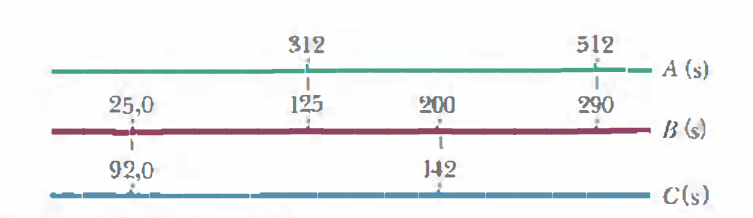
\includegraphics[scale=0.5]{images/hal13.png}
			\caption{Leitura simultânea de pares de relógios em quatro ocasiões (relógios A, B e C).}
		\end{figure}
	\end{center}
	
	\item {\bf (Halliday 1.21)} 
		\begin{enumerate}
			\item Supondo que a água tenha uma massa específica de exatamente 1 g/$\mbox{cm}^3$, determine a massa de um metro cúbico de água em quilogramas.
			\item Suponha que sejam necessárias 10,0 h para drenar um recipiente com 5700 $m^3$ de água. Qual é a ``vazão mássica'' da água do recipiente, em quilogramas por segundo?
		\end{enumerate}		 
\section{Programação}
	
	\item Em JavaScript, crie um protótipo de objeto {\tt Carro} que tenha as propriedades (i) {\tt placa}, (ii) {\tt cor}, (iii) {\tt velocidadeMaxima}, e (iv) {\tt relatorio}. A {\tt placa} e a {\tt cor} são cadeias; a {\tt velocidadeMaxima} é um número fracionário; e {\tt relatorio} é uma função que exibe, via {\tt console.log}, todas as demais propriedades de {\tt Carro}. Crie um objeto a partir de {\tt Carro}. Atribua valores para as propriedades ao seu gosto. 
	
	\vspace{0.3cm}
	
	{\color{blue} Resposta: }

	\begin{lstlisting}[language=JavaScript]
function Carro(placa, cor, velocidadeMaxima){
	this.placa = placa;
	this.cor = cor;
	this.velocidadeMaxima = velocidadeMaxima;
	this.relatorio = function(){
		console.log("===RELATORIO===");
		console.log("Placa: " + this.placa);
		console.log("Cor: " + this.cor);
		console.log("Velocidade Maxima: " + this.velocidadeMaxima);
	};
}

carro1 = new Carro("PQT-4567", "preto", 180.45);
carro1.relatorio();	//exibe os dados do objeto carro1
\end{lstlisting}
	
	\item Em JavaScript, crie um protótipo de objeto {\tt Calculadora} que tenha as propriedades de {\tt somar}, {\tt dividir}, {\tt subtrair} e {\tt multiplicar}. Todas estas propriedades são operações binárias, recebem valores inteiros e retornam valores inteiros. Se, para as entradas fornecidas, não for possível gerar um valor de retorno válido, então exiba, via {\tt console.log}, o motivo do não retorno do valor.
		
\end{enumerate}

\section{Referências}

\begin{itemize}
	\item HALLIDAY, D.; RESNICK, R.. Fundamentos de Física. Volume 1, Mecânica. 8ª Edição, LTC, Rio de Janeiro, 2011.

	\item RAMTAL, D.; DOBRE, A. Physics for JavaScript Games, Animation, and Simulations with HTML5 Canvas, Apress, 2014.
\end{itemize}

\end{document}